% ICEIR 2026 -- Springer LNCS (llncs class), revised version after review (Paper 282). Compile on Overleaf with pdfLaTeX.
% Results: code/results/iceir/ and code/results/iceir/rev1/ (code/src/review_iceir_rev1.py); figures: make_figures_rev1.py
\documentclass[runningheads]{llncs}
\usepackage[T1]{fontenc}
\usepackage[utf8]{inputenc}
\usepackage{graphicx}
\usepackage{cite}
\usepackage{microtype}
\usepackage{booktabs}
\usepackage{amsmath,amssymb}
\usepackage{array}
\usepackage{float}
\usepackage{placeins}
\usepackage{tikz}
\usetikzlibrary{arrows.meta,positioning}
\usepackage[hidelinks]{hyperref}
\graphicspath{{figures/}}
\providecommand{\doi}[1]{\url{https://doi.org/#1}}

\begin{document}
\setlength{\emergencystretch}{1.5em}

\title{Reproducing or Predicting? Regulation-Grounded Evaluation of Debt-Group Classification and Early Warning in a Vietnamese Commercial Bank}
\titlerunning{Reproducing or Predicting Debt-Group Migration?}

\author{Le Thi Thanh An\inst{1,2} \and
Le Kim Thu\inst{3} \and
Dam Cong Danh\inst{3}\thanks{Corresponding author.}}
\authorrunning{T. T. A. Le, K. T. Le, and C. D. Dam}
\institute{University of Economics and Law, Ho Chi Minh City, Vietnam \and
Vietnam National University, Ho Chi Minh City, Vietnam \and
School of Applied Mathematics and Informatics, Hanoi University of Science and Technology, No.~1 Dai Co Viet, Hanoi, Vietnam\\
\email{danh.dc251317M@sis.hust.edu.vn}}

\maketitle

\begin{abstract}
Machine-learning models of bank credit risk are often judged by how well they reproduce the current debt group on a random split of one snapshot. Using two consecutive monthly snapshots (April and May 2026; about 100,000 loans each) of a Vietnamese commercial bank, we examine what such evaluations miss. First, two interest fields that accounting rules record according to the debt group inflate five-class Macro-F1 from 0.43 to 0.69, mostly through off-balance-sheet unpaid interest. Under decile binning this field has an Information Value (IV) of zero; a separate zero bin flags it, but flags an innocent field as well, so only its regulatory provenance identifies it as leakage. Second, splitting the out-of-time snapshot by contract overlap shows that apparent temporal stability is partly an artefact: without the interest fields, Macro-F1 is 0.49 on contracts seen in training and 0.40 on unseen ones, and an apparent 13--32\% decline was traced to a silent date-encoding change. Third, for 31-day migration to a worse group (0.27\% of loans), 83\% of events are mechanical crossings of the regulation's days-past-due (DPD) thresholds. Because all contracts of a customer share one group, contract-level cross-validation overstates early-warning performance; with customer-grouped folds, the average precision (AP) of gradient boosting without overdue fields falls from 0.18 to 0.03. A rule ranking loans by distance to the next threshold reaches AP 0.21; a model given the same information (DPD and current group) reaches 0.29 and finds 64\% of migrations in the top 1\% of loans, against 48\% for the rule.

\keywords{Credit risk \and Early warning \and Data leakage \and Out-of-time validation \and Regulatory baseline \and Recall@k.}
\end{abstract}

% ---------------------------------------------------------------------------
\section{Introduction}
\label{sec:intro}

Vietnamese commercial banks must classify every loan into one of five debt groups of increasing risk, with groups 3--5 constituting non-performing debt. The framework in force is Circular 31/2024/TT-NHNN as amended by Circular 37/2025/TT-NHNN~\cite{sbv2024tt31}, which retains the five-group structure of Circular 11/2021/TT-NHNN~\cite{sbv2021tt11} and sets days-past-due (DPD) thresholds of 10, 90, 180 and 360 days between consecutive groups. The group determines specific provisioning under Decree 86/2024/ND-CP~\cite{gov2024nd86} and interest-income recognition under Decree 135/2025/ND-CP~\cite{gov2025nd135}. Machine learning (ML) is increasingly proposed to support this process, and benchmarking studies consistently place tree ensembles among the strongest methods on tabular credit data~\cite{lessmann2015benchmarking,brown2012experimental}.

Studies of this kind, including several for Vietnamese banks~\cite{tran2021mlcredit,trung2024credit,nguyen2024ews}, typically report accuracy, F1 or the area under the receiver operating characteristic curve (ROC-AUC). When the target is the debt group and evaluation uses a random split of one reporting snapshot, three questions remain open: whether the inputs are admissible given how they are produced, whether an out-of-time (OOT) test truly measures performance on unseen loans, and whether a model predicts more than the regulation's own DPD thresholds already imply. We examine them on two consecutive monthly snapshots of a Vietnamese commercial bank (100,617 and 100,274 contracts). The contributions are:

\begin{itemize}
\item[\textbf{C1}] A \emph{regulation-grounded leakage audit} with a field-level register (Appendix~\ref{app:register}). Two interest fields that Decree 135/2025/ND-CP records according to the label inflate five-class Macro-F1 from 0.43 to 0.69. The main one has an IV of zero under decile binning and is flagged by a well-binned IV only together with an innocent field; its shifting relation to the label also causes systematic out-of-time errors.
\item[\textbf{C2}] An \emph{overlap-aware evaluation} that separates next-month contracts, and customers, seen in training from unseen ones. It shows that the usual OOT figure overstates temporal transfer and that contract-level cross-validation overstates the average precision of early-warning models two- to sevenfold; between-extract integrity checks also exposed a silent date-encoding change that produced a spurious 13--32\% decline.
\item[\textbf{C3}] \emph{Regulatory baselines for early warning under information parity}, evaluated as budget-constrained retrieval. Migration is decomposed into mechanical DPD-threshold crossings and other events, and ML models given the same information as a distance-to-threshold rule are compared with it, with a scorecard and with a learning-to-rank objective, using customer-grouped Recall@k, AP, severity-weighted NDCG, dependence-corrected tests and a provision-weighted choice of the review budget.
\end{itemize}

\paragraph{Relation to our prior work.} An earlier paper by the same authors~\cite{an2026sebl}, presented at the UEL SEBL 2026 conference on 6 October 2026, used a different extract from the same bank (one undated snapshot of 27,001 contracts and 21 columns from around 2020) and addressed only five-class classification with a random split. The present paper uses two dated 2026 snapshots with 33 columns, adds the migration task, overlap-aware evaluation and regulatory baselines, and reuses no result from~\cite{an2026sebl}.

% ---------------------------------------------------------------------------
\section{Related Work}
\label{sec:related}

\subsection{Machine Learning for Credit Scoring}

Large benchmarks~\cite{baesens2003benchmarking,lessmann2015benchmarking} find that ensembles perform well on average but that rankings depend on the dataset and metric, and the best algorithm changes with class imbalance~\cite{brown2012experimental}. Gradient boosting (XGBoost~\cite{chen2016xgboost}, LightGBM~\cite{ke2017lightgbm}, CatBoost~\cite{prokhorenkova2018catboost}) dominates recent tabular work. In Vietnam, Nguyen and Ngo~\cite{nguyen2025boosting} compare AdaBoost, XGBoost, LightGBM and CatBoost for personal default on 7,542 customers (2014--2022, 12 features) and find LightGBM best. Nguyen et al.~\cite{nguyen2024ews} build an early-warning system for debt-group migration at one bank with logistic regression, support vector machine (SVM), decision tree and random forest: random forest reaches the highest accuracy (81.84\%) for migration into overdue debt, SVM the highest recall (91.48\%, at 46.62\% accuracy), and performance declines on new data. Further Vietnamese studies~\cite{tran2021mlcredit,trung2024credit} likewise evaluate classifiers at a fixed threshold.

\subsection{Leakage, Dataset Shift and Ranking Evaluation}

Leakage is the use of information not legitimately available at prediction time~\cite{kaufman2012leakage}. In scorecard practice, IV is the standard univariate screen: an IV of 0.3 or more is rated strong~\cite{siddiqi2006credit}, and much higher values (e.g., above 0.5 or 1.0) prompt a leakage check. IV contrasts good and bad loans after binning, so its value depends on the binning: under plain quantile binning a zero-inflated field can collapse into a single bin, which coarse classing avoids by giving such values a bin of their own~\cite{siddiqi2006credit}. Out-of-time samples are the usual safeguard against dataset shift~\cite{siddiqi2006credit,morenotorres2012unifying}. For early warning, Khandani et al.~\cite{khandani2010consumer} forecast consumer delinquency months ahead from transaction and credit-bureau data, and rating-migration studies estimate transition probabilities between grades~\cite{lando2002analyzing}. With rare positives, precision--recall measures such as AP are more informative than ROC analysis~\cite{saito2015precision}. Recall@k, the share of events found in the top $k\%$ of a ranking, equals the capture rate read from the cumulative gains (lift) chart and is the ordinate of the cumulative accuracy profile (CAP) used in scorecard and rating validation~\cite{siddiqi2006credit,engelmann2003testing}; treating a review queue with a fixed budget as retrieval adds rank-sensitive measures that weight its top, such as AP and normalised discounted cumulative gain (NDCG), and learning-to-rank objectives. Comparisons across resampled folds need the variance correction of Nadeau and Bengio~\cite{nadeau2003inference}. SHapley Additive exPlanations (SHAP)~\cite{lundberg2017unified,lundberg2020tree} are widely used to explain credit models~\cite{bussmann2021explainable}.

\subsection{Research Gap}
\label{sec:gap}

\paragraph{G1: leakage is screened statistically, not by provenance.} In Vietnamese bank data several reporting fields, such as specific provisions and off-balance-sheet interest, are \emph{produced} from the debt group by provisioning and accounting rules~\cite{gov2024nd86,gov2025nd135}. To our knowledge, no published study judges input admissibility by the regulatory process that generates each field. Section~\ref{sec:leak} shows that a decile-binned IV screen misses such a field entirely, and that even a well-binned screen flags it together with an innocent field: IV measures association, not provenance.

\paragraph{G2: evaluations ignore contract and customer overlap.} Consecutive monthly snapshots contain largely the same loans, and the classification rules assign all contracts of a customer to one group~\cite{sbv2024tt31}. A next-month test set therefore overlaps the training data, and a contract-level split places contracts of one customer, with the same label, on both sides. We are not aware of credit-scoring studies that separate seen from unseen contracts or customers when reporting performance.

\paragraph{G3: early warning lacks regulatory baselines.} Early-warning studies compare ML models with one another at fixed thresholds~\cite{nguyen2024ews}. Because migration between groups is largely defined by DPD thresholds, the relevant benchmark is the ranking already implied by the regulation, compared with models that receive the same information and evaluated under a review budget. G1--G3 correspond to C1--C3.

% ---------------------------------------------------------------------------
\section{Data and Problem Formulation}
\label{sec:data}

\subsection{Data}

The data are two monthly credit-information extracts of the same bank's loan book, with an identical 33-column schema based on the State Bank of Vietnam reporting template: 30 April 2026 (100,617 contracts) and 31 May 2026 (100,274 contracts). The target is the bank's self-assessed debt group (Table~\ref{tab:dist}). Group~1 is 89 times larger than group~3, but the rare groups remain large enough in absolute terms for per-group evaluation. Of the April contracts, 98,968 also appear in May; 1,306 May contracts are new.

\begin{table}[t]
\centering
\caption{Debt-group distribution in the two snapshots.}
\label{tab:dist}
\small
\begin{tabular}{@{}lrrrrrr@{}}
\toprule
& G1 & G2 & G3 & G4 & G5 & Total\\
\midrule
30/04/2026 & 88,875 & 6,321 & 998 & 1,446 & 2,977 & 100,617\\
\quad share (\%) & 88.33 & 6.28 & 0.99 & 1.44 & 2.96 & 100.00\\
31/05/2026 & 88,527 & 6,339 & 991 & 1,421 & 2,996 & 100,274\\
\quad share (\%) & 88.28 & 6.32 & 0.99 & 1.42 & 2.99 & 100.00\\
\bottomrule
\end{tabular}
\end{table}

\subsection{Two Tasks}

Table~\ref{tab:tasks} defines the two tasks. Task~1 \emph{reproduces} the current group from fields of the same snapshot; Task~2 \emph{predicts} whether loan $i$ moves to a worse group within 31 days, $Y_i=\mathbb{I}(G_{i,T+h}>G_{i,T})$ with $T=$ 30 April 2026 and $h=31$ days, using only fields observed at $T$. All 265 migrations move by exactly one group (214 from group 1 to 2, 10 from 2 to 3, 10 from 3 to 4 and 31 from 4 to 5), so a rule predicting no migration is 99.73\% accurate and the task is treated as ranking a review queue.

\begin{table}[t]
\centering
\caption{The two tasks. OOT: out-of-time; CV: cross-validation; AP: average precision.}
\label{tab:tasks}
\scriptsize
\begin{tabular}{@{}>{\raggedright\arraybackslash}p{1.7cm}>{\raggedright\arraybackslash}p{4.6cm}>{\raggedright\arraybackslash}p{5.3cm}@{}}
\toprule
& Task 1: reproduce the current group & Task 2: predict 31-day migration\\
\midrule
Unit & Contract in a snapshot & Contract present at $T$ and $T+h$ (98,968)\\
Label & Debt group 1--5 (multi-class) & Moves to a worse group by $T+h$ (265 events, 0.27\%)\\
Inputs & 18 fields of the same snapshot in the main (conservative) configuration; 20 with the two interest fields (Sect.~\ref{sec:leak}) & The 20 fields at $T$, plus overdue amounts, DPD and the current group $G_T$\\
Training / evaluation & 80/20 stratified split of April, by contract and by customer; all of May as OOT, split by overlap & Stratified 5-fold CV repeated 10 times (50 folds), grouped by customer\\
Primary measure & Macro-F1 & AP; Recall@k and Precision@k for a review budget of $k\%$\\
\bottomrule
\end{tabular}
\end{table}

% ---------------------------------------------------------------------------
\section{Methodology}
\label{sec:method}


\subsection{Data Preparation and Integrity}
\label{sec:prep}

\paragraph{A silent date-encoding defect.} In our first out-of-time run, every model appeared to deteriorate markedly in May, with relative Macro-F1 declines from 12.7\% (logistic regression) to 32.1\% (CatBoost). The cause was a data defect, not dataset shift: the April extract stores disbursement and contract end dates as \texttt{yyyymmdd} integers, whereas the May extract stored them as Excel serial numbers (e.g., 45965 for 4 November 2025). The parser recognised only the former and silently returned empty values, so the three date-derived features were 100\% missing in the OOT set and were imputed with training medians. A between-extract comparison of missing rates exposed the problem. After the dates were standardised at source, the apparent degradation disappeared and the median loan age rose by one month (395 to 426 days), as expected; the parser now rejects any other format, and all results below use the corrected data.

\paragraph{Joining and partitioning.} Snapshots are joined on the contract key. The 1,649 April contracts absent in May (settled, written off or re-registered; the data do not say which) have no migration label; 97.3\% of them are in group~1, and a sensitivity analysis counts exits from groups 2--5 as events. May contracts are partitioned into those in the April training split (79,144), in the April test split (19,824) and new (1,306). Feature stability between snapshots is measured by the population stability index (PSI); once the three restructuring fields are set to zero for never-restructured loans, no feature has missing values in either snapshot.

\paragraph{Customer structure.} The April snapshot has 73,494 customers (1.37 contracts per customer, at most 313). Customers with more than one contract are 16.9\% of customers but hold 39.3\% of contracts, and none of them has contracts in different groups, as the classification rules require~\cite{sbv2024tt31}. Under a contract-level split, 35.7\% of test contracts therefore belong to a customer whose other contracts, with the same label, are in the training data. We report Task~1 under both contract-level and customer-grouped splits, and evaluate Task~2 with customer-grouped folds only.

\subsection{Regulation-Grounded Leakage Audit (C1)}
\label{sec:leak}

Every field is classified by the process that writes it (Table~\ref{tab:audit}; full register in Appendix~\ref{app:register}).

\begin{table}[t]
\centering
\caption{Three-layer leakage audit of the 33 fields. CIC: National Credit Information Centre.}
\label{tab:audit}
\scriptsize
\begin{tabular}{@{}>{\raggedright\arraybackslash}p{1.9cm}>{\raggedright\arraybackslash}p{4.3cm}>{\raggedright\arraybackslash}p{5.4cm}@{}}
\toprule
Layer & Fields & Decision and basis\\
\midrule
1. Label restatements (7) & CIC-reconciled group; overdue principal and interest amounts and their overdue dates; specific provisions required and booked & Excluded in Task~1: alternative label, direct classification criteria (DPD thresholds~\cite{sbv2024tt31}), or provisions computed from the group (rates 0/5/20/50/100\%~\cite{gov2024nd86}). Overdue fields re-enter Task~2 as states at $T$.\\
2. Identifiers, duplicates, constants (6) & Customer and contract identifiers (4); recovery date ($=$ contract end date); paid amount (always 0) & Excluded: no information\\
3. Rule-grounded review & Off-balance-sheet unpaid interest; on-balance-sheet interest receivable & Recorded by group under Art.~13(2)(a) of Decree 135/2025/ND-CP~\cite{gov2025nd135}; quantified by ablation; excluded from the main Task-1 configuration\\
\bottomrule
\end{tabular}
\end{table}

The Layer-3 evidence is regulatory, not merely statistical. Article~13(2)(a) of Decree 135/2025/ND-CP, in force at both snapshot dates (it superseded Circular 16/2018/TT-BTC and was amended by Decree 316/2026/ND-CP only after them), lets banks recognise accrued interest as revenue only for loans classified as standard; interest on other loans, and on loans kept in the standard group under state policy, is monitored off balance sheet~\cite{gov2025nd135}. Accordingly, off-balance-sheet interest is positive for 0.01\% of group-1 loans but for 21.5\%, 78.1\%, 93.0\% and 97.2\% of groups 2--5 in April. IV is computed on April with ``bad'' defined as groups 2--5 and ``good'' as group~1 (11,742 against 88,875 loans). Under decile binning the field's IV is 0.000: 93.6\% of its values are zero, all decile edges coincide and every record falls into one bin. With a separate bin for zero, as coarse classing prescribes, its IV is 5.09 and the field is flagged; but the same screen also flags loan age (1.12), which more plausibly reflects seasoning, and rates on-balance-sheet interest 0.85. IV therefore depends on the binning and, even when well binned, measures association rather than provenance: it cannot tell a field recorded \emph{from} the label apart from a strong legitimate predictor, whereas the regulation can. The main Task-1 results therefore use the \emph{conservative} configuration without both interest fields; the full configuration measures the inflation due to leakage. In Task~2 the interest and overdue fields describe the state at $T$, before the event, and are admissible provided they are not revised retroactively.

\subsection{Models, Baselines and Evaluation}
\label{sec:eval}

Six learners are compared: logistic regression (LR), decision tree (DT; depth 10), random forest (RF; 300 trees), XGBoost (XGB) and LightGBM (LGBM) (400 trees, learning rate 0.05, depth 6 and 8 respectively) and CatBoost (CB; 400 iterations, with balanced class weights instead of SMOTE because its categorical inputs cannot be interpolated). Hyper-parameters are fixed a priori at common library-style values; a 12-configuration grid is used only as a sensitivity check on the internal test split, and the May snapshot is never used for any choice. Four imbalance strategies are compared (none, class weights, moderate synthetic minority over-sampling (SMOTE)~\cite{chawla2002smote} and both); all preprocessing and resampling are fitted inside each training fold within an \texttt{imblearn} pipeline. Twenty features remain after Layers 1--2 (12 numeric, 8 categorical, including loan age, days to maturity, actual tenor and a restructuring flag engineered from the dates); the main Task-1 configuration drops the two Layer-3 interest fields and uses 18.

For Task~2, the main model is XGB on the 20 features, four overdue fields at $T$ (principal and interest DPD and amounts) and the current group $G_T$. To separate what each input contributes, XGB is also fitted on the 20 features alone, on the 20 features plus $G_T$, on the 20 features plus the overdue fields, and on the full set plus the rule score as a feature. The models are compared with: (i) a rule ranking loans by their distance to the next DPD threshold (10, 91, 181 and 361 days for groups 1--4), which uses DPD and $G_T$ and needs no training; (ii) DPD alone; (iii) univariate rankings by each interest field; and, all on the full information set, (iv) a logistic scorecard on weight-of-evidence (WOE) bins~\cite{siddiqi2006credit}, (v) XGB with a pairwise learning-to-rank objective, with each training fold as a single query so that every event is paired with every non-event, and (vi) LGBM, RF, DT and LR. A migration is \emph{mechanical} if the loan is overdue at $T$ and will cross the next DPD threshold within 31 days if unpaid. Task-2 rankings are evaluated by stratified 5-fold cross-validation repeated 10 times with folds grouped by customer, so that no customer appears in both training and test data; contract-level figures are reported only to show the difference. Task-1 models are scored by Macro-F1; Task-2 rankings by AP (random level 0.0027), Recall@k and Precision@k, and NDCG@5\% with gain equal to the origin group (a 4$\to$5 migration weighs four times a 1$\to$2 one), all as mean $\pm$ standard deviation over the 50 folds. Differences in AP are tested with the corrected resampled $t$-test~\cite{nadeau2003inference}, with Holm adjustment for the learner comparison. SHAP values use path-dependent TreeSHAP~\cite{lundberg2020tree}, which needs no background sample, on a label-stratified (event-oversampled) sample of all 53 test events and 447 non-events from a customer-grouped 80/20 split.


% ---------------------------------------------------------------------------
\section{Results}
\label{sec:results}

\subsection{Task 1: Leakage Inflation and Overlap-Aware Out-of-Time Performance}

Table~\ref{tab:task1} gives the two leading learners in both configurations. In the conservative (main) configuration, LGBM and XGB reach Macro-F1 0.429 and 0.423 on the internal test split. With all 20 fields they also lead (0.693 and 0.694), ahead of RF (0.662), DT (0.657), CB (0.601) and LR (0.403); the gap between the leaders is smaller than each model's range over its hyper-parameter grid (0.096 and 0.056).

\begin{table}[t]
\centering
\caption{Task 1, Macro-F1. Conservative: 18 fields, without both interest fields (main result); full: all 20 fields (leakage-inflated). (a) Contract-level 80/20 split of April; May contracts are split by whether they were in the training split (seen), the test split (unseen) or are new (not shown). Brackets: 95\% customer-cluster bootstrap intervals (1,000 resamples). (b) Customer-grouped 80/20 split; May contracts are split by whether their customer is in the training data. Bold: main results.}
\label{tab:task1}
\scriptsize
\setlength{\tabcolsep}{3pt}
\begin{tabular}{@{}llcccc@{}}
\toprule
\multicolumn{6}{@{}l}{(a) Contract-level split} \\
& & Internal test & May, seen & May, unseen & May, all\\
& & ($n=20{,}124$) & ($n=79{,}144$) & ($n=19{,}824$) & ($n=100{,}274$)\\
\midrule
Conservative & LGBM  & 0.429 & 0.490 & \textbf{0.404} & 0.473\\
 & & {\tiny [0.410, 0.447]} & {\tiny [0.479, 0.500]} & {\tiny [0.389, 0.418]} & {\tiny [0.463, 0.482]}\\
 & XGB  & 0.423 & 0.466 & \textbf{0.407} & 0.455\\
 & & {\tiny [0.406, 0.440]} & {\tiny [0.456, 0.477]} & {\tiny [0.392, 0.422]} & {\tiny [0.445, 0.463]}\\
Full (leaky) & LGBM  & 0.693 & 0.714 & 0.635 & 0.698\\
 & & {\tiny [0.675, 0.713]} & {\tiny [0.706, 0.722]} & {\tiny [0.618, 0.652]} & {\tiny [0.691, 0.706]}\\
 & XGB  & 0.694 & 0.697 & 0.637 & 0.685\\
 & & {\tiny [0.676, 0.714]} & {\tiny [0.688, 0.706]} & {\tiny [0.618, 0.654]} & {\tiny [0.677, 0.693]}\\
\midrule
\multicolumn{6}{@{}l}{(b) Customer-grouped split} \\
& & Internal test & May, customer seen & May, customer unseen & May, all\\
& & ($n=20{,}124$) & ($n=79{,}711$) & ($n=20{,}563$) & ($n=100{,}274$)\\
\midrule
Conservative & LGBM & 0.419 & 0.502 & \textbf{0.413} & 0.484\\
 & XGB & 0.417 & 0.467 & \textbf{0.412} & 0.455\\
Full (leaky) & LGBM & 0.665 & 0.726 & 0.620 & 0.705\\
 & XGB & 0.668 & 0.702 & 0.629 & 0.687\\
\bottomrule
\end{tabular}
\end{table}

\paragraph{Leakage inflation.} The interest fields raise Macro-F1 from 0.43 to 0.69 on the internal test split; off-balance-sheet interest alone accounts for 54.8\% of LGBM's total Gain importance (the loss reduction from splits on a field) and 31.3\% of its SHAP importance. Without it, Macro-F1 is 0.479; without both fields, 0.429. Off-balance-sheet interest thus accounts for most (0.21 of 0.26) but not all of the inflation; on-balance-sheet interest, recorded under the same article, contributes the rest. 

\paragraph{Overlap.} The usual OOT figure (all of May) suggests no loss: 0.698 against 0.693 internally. Split by overlap, the seen contracts score 0.714 and the unseen 0.635 ($-8\%$ relative to the internal 0.693); in the conservative configuration, 0.490 against 0.404 ($-6\%$ relative to the internal 0.429). The bootstrap intervals of seen and unseen contracts do not overlap in either configuration. Grouping the split by customer changes little (Table~\ref{tab:task1}b): the conservative LGBM scores 0.419 internally and 0.413 on May contracts of customers absent from training, so customer overlap does not drive the Task-1 conclusions. The 1,306 new contracts are almost all in group~1 (1,304) and support only an accuracy check (0.995). PSI is below 0.05 for every feature, yet it misses a shift that matters: in May, 1,092 group-1 loans carry off-balance-sheet interest (1.23\% of group~1, against 0.01\% in April), 1,091 of them already in group~1 in April, whereas the shares for groups 2--5 (19.5\%, 78.6\%, 93.5\% and 97.4\%) stay close to April's. The full LGBM classifies 835 of them as group~4, which accounts for \emph{all} its group-1-to-group-4 errors. The pattern is consistent with the policy exception in Art.~13(2)(a) and shows that a regulation-produced field can change meaning between extracts while its marginal distribution stays stable.

\paragraph{Per-group behaviour and robustness.} Without the interest fields, group~2 is almost never recognised (recall 0.03, against 0.20 in the full configuration) and 3.0\% of internal predictions are off by two or more groups (0.4\% in the full configuration). In the conservative configuration, Macro-F1 is unchanged without resampling (0.429), lower with class weights (0.377) or class weights plus SMOTE (0.388), and within 0.013 of the main result with SMOTE for nominal and continuous features (SMOTE-NC; 0.442 for LGBM, 0.425 for XGB), categorical branch coding (0.430 and 0.420) and the eight features with the highest Gain (0.433). Gain and SHAP rank the six feature groups similarly (Spearman $\rho=0.83$, $p=0.042$). The full configuration gives the same conclusions.

\subsection{Task 2: Regulatory Baselines for Early Warning}

Of the 265 migrations, 220 (83\%) are mechanical. They occur in 181 customers, and 119 of them belong to customers with two or more migrating contracts. Table~\ref{tab:task2} and Fig.~\ref{fig:recall} compare the rankings.

\begin{table}[t]
\centering
\caption{Task 2, 31-day migration (98,968 loans, 265 events): mean over 50 customer-grouped folds ($\pm$ sd for AP; for the sd of Recall@k see Fig.~\ref{fig:recall}; fold sd of P@5\% is at most 0.006, 0.014 for the scorecard). AP$^{\mathrm{c}}$: AP under contract-level folds, shown to quantify the effect of customer overlap (--: not run with the same inputs). R@k, P@k: Recall@k and Precision@k; NDCG weighted by origin group. Full information: 20 features, overdue fields and $G_T$.}
\label{tab:task2}
\scriptsize
\setlength{\tabcolsep}{2.2pt}
\resizebox{\textwidth}{!}{%
\begin{tabular}{@{}lccccccc@{}}
\toprule
Method & AP & ROC-AUC & R@1\% & R@5\% & P@5\% & NDCG@5\% & AP$^{\mathrm{c}}$\\
\midrule
XGB, full information (main) & \textbf{0.292 $\pm$ 0.059} & \textbf{0.926} & \textbf{0.637} & 0.823 & 0.044 & \textbf{0.562} & 0.483\\
\quad + rule score as feature & 0.417 $\pm$ 0.055 & 0.927 & 0.693 & 0.819 & 0.044 & 0.748 & 0.576\\
Rule: distance to threshold & 0.206 $\pm$ 0.041 & 0.894 & 0.479 & \textbf{0.840} & \textbf{0.045} & 0.485 & 0.203\\
XGB + overdue fields (no $G_T$) & 0.203 $\pm$ 0.040 & 0.924 & 0.548 & 0.817 & 0.044 & 0.531 & 0.393\\
XGB pairwise, full information & 0.176 $\pm$ 0.080 & 0.914 & 0.466 & 0.695 & 0.037 & 0.321 & --\\
XGB, 20 features + $G_T$ & 0.044 $\pm$ 0.020 & 0.800 & 0.198 & 0.388 & 0.021 & 0.300 & 0.207\\
WOE scorecard, full information & 0.027 $\pm$ 0.027 & 0.799 & 0.132 & 0.334 & 0.018 & 0.193 & --\\
XGB, 20 features & 0.026 $\pm$ 0.015 & 0.776 & 0.131 & 0.334 & 0.018 & 0.209 & 0.179\\
DPD at $T$ & 0.017 $\pm$ 0.003 & 0.872 & 0.000 & 0.178 & 0.010 & 0.138 & 0.017\\
On-balance interest & 0.005 $\pm$ 0.001 & 0.620 & 0.019 & 0.073 & 0.004 & 0.019 & 0.004\\
Off-balance interest & 0.004 $\pm$ 0.001 & 0.564 & 0.008 & 0.180 & 0.010 & 0.141 & 0.004\\
\bottomrule
\end{tabular}}
\end{table}

\begin{figure}[t]
\centering
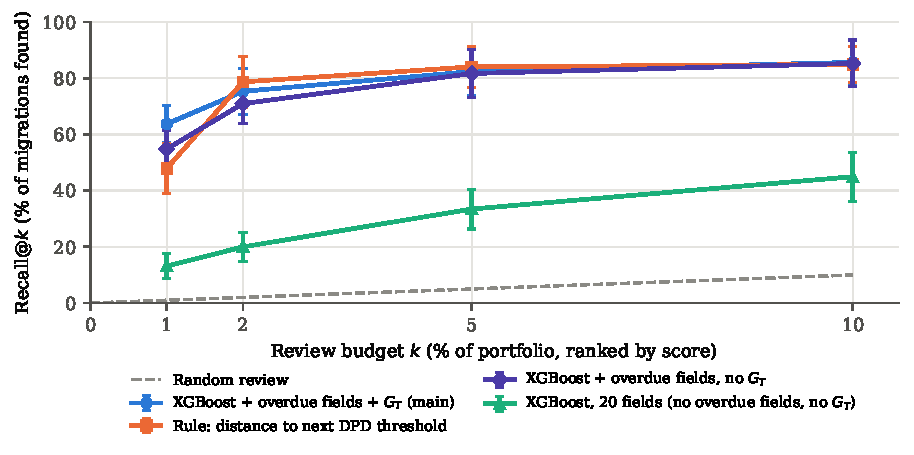
\includegraphics[width=0.86\textwidth]{fig2_recall_at_k_rev1.pdf}
\caption{Recall@k (mean $\pm$ sd over 50 customer-grouped folds) by review budget. $G_T$: current debt group; DPD: days past due.}
\label{fig:recall}
\end{figure}

\paragraph{Customer overlap inflates contract-level results.} Contract-level folds let a model recognise a customer whose other contracts migrate in the training data. With customer-grouped folds, the AP of XGB on the 20 features falls from 0.179 to 0.026 and that of XGB with overdue fields from 0.393 to 0.203, whereas the untrained rule is unaffected (0.206). Contract-level evaluation would thus suggest that the rule merely matches a model without overdue fields; under customer-grouped evaluation, models without DPD are far below it (AP 0.026--0.044; corrected $p<0.001$).

\paragraph{What ML adds under the same information.} The rule uses DPD and $G_T$. Given the overdue fields but not $G_T$, XGB ties with the rule (AP 0.203 against 0.206; $p=0.91$). Given both, it exceeds the rule (0.292; $p=0.004$), raises Recall@1\% from 48\% to 64\% and NDCG@5\% from 0.48 to 0.56, while Recall@5\% is similar (82\% against 84\%). The gain is therefore precision at the very top of the queue; at a 5\% budget, about 23 loans are reviewed per migration found (Precision@5\% $=0.044$). Adding the rule score as a feature raises AP further to 0.417 ($p<0.001$): the regulation's own ranking is also a valuable input to the model. For the 45 non-mechanical migrations all methods are weak: AP is 0.012--0.026 for the XGB models against a base rate of 0.0005, but with about nine events per fold the fold standard deviations (0.03--0.06) exceed the means, so this signal cannot be distinguished from noise.

\paragraph{Choosing the review budget.} Weighting each migration by the increase in specific provision it triggers (the difference between the rates of Decree 86/2024/ND-CP for the new and the old group times the outstanding balance; all 265 migrating loans are in VND, and amounts are in million VND), the top 1\% of the out-of-fold queue of the main model captures 57\% of the total, against 50\% for the rule; at 5\% the shares are 74\% and 67\%. The provision at stake per reviewed loan is about VND 16 million in the top 1\%, but each loan reviewed beyond 5\% adds less than VND 0.05 million. Unless reviews are almost free relative to the provisions they anticipate, a budget between 1\% and 5\% is the defensible choice; the bank's own cost per review fixes the point within this range.

\paragraph{Ranking objective, scorecard and learners.} With the full information set, the pairwise learning-to-rank objective is worse than binary classification (AP 0.176 against 0.292, $p=0.012$), and the WOE scorecard is much worse (0.027). Among the learners (best of no resampling and moderate SMOTE per learner, i.e., a best-of-strategy estimate; CatBoost was not rerun under the grouped protocol because of its run time), LGBM with SMOTE (0.323), RF (0.310) and XGB (0.292) are statistically tied (Holm-adjusted $p\ge0.29$), whereas a naive Wilcoxon test would separate LGBM and XGB ($p<0.001$); DT (0.253; $p=0.051$) and LR (0.006) are worse. XGB is kept as the main model for comparability with the other rows of Table~\ref{tab:task2}.

\paragraph{Admissibility and selection sensitivity.} Removing off-balance-sheet interest, or both interest fields, from the main model leaves AP unchanged (0.295 and 0.293 against 0.292; corrected $p\ge0.71$), so the early-warning results do not depend on the admissibility of the interest fields. Counting the 45 exits from groups 2--5 as events lowers AP to 0.234. In the main model, the most influential inputs by mean absolute SHAP are interest DPD (mean $|\phi|=1.93$), the current group (0.53), actual tenor (0.52), outstanding balance (0.49) and days to maturity (0.44) (Fig.~\ref{fig:shap}). The largest positive contributions go to loans with short but positive interest DPD, consistent with proximity to the 10-day threshold, and high current groups push scores down because group-5 loans cannot migrate; the same values could supply reason codes for individual alerts.

\begin{figure}[t]
\centering
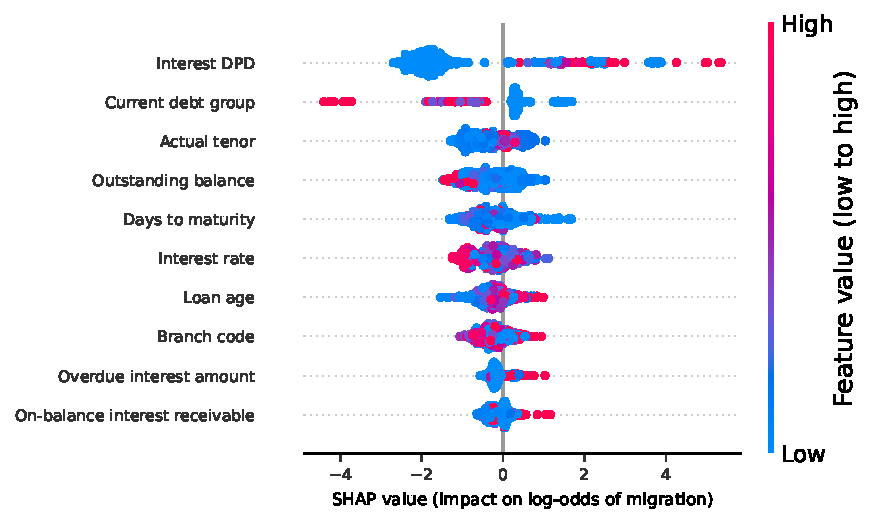
\includegraphics[width=0.66\textwidth]{fig3_shap_beeswarm_rev1.pdf}
\caption{SHAP values of the main Task-2 model (XGB with full information) on the label-stratified sample of 53 events and 447 non-events from a customer-grouped split; ten most influential inputs. Colour: feature value (not meaningful for the categorical branch code); DPD: days past due.}
\label{fig:shap}
\end{figure}

% ---------------------------------------------------------------------------
\section{Discussion}
\label{sec:discussion}

\paragraph{Reproducing versus predicting.} The two tasks give different answers to the same question. A five-class model appears strong (Macro-F1 0.69) only because accounting fields restate the label; without them it reaches 0.43, and 0.40 on unseen next-month contracts. A migration model without overdue fields appears useful under contract-level folds (AP 0.18), but most of that signal comes from customers whose other contracts are in the training data: with customer-grouped folds it falls to 0.03, far below a rule derived from the classification regulation. ML adds value only when it receives the information the rule uses, DPD and the current group, and then mainly by sharpening the top of the review queue. In both tasks, the regulation itself explains much of what the model learns.

\paragraph{Regulation as leakage source and as baseline.} The decisive leakage evidence came from Decree 135/2025/ND-CP rather than from a statistical screen. With decile binning, the most influential leaking field has an IV of zero and only loan age, which reflects seasoning, exceeds the alert level; with a separate zero bin, the leaking field is flagged (IV 5.09), but so is loan age. A statistical screen, however binned, ranks fields by association with the label and cannot establish the direction or timing of a dependence. Likewise, the decisive baseline came from Circular 31/2024/TT-NHNN rather than from another learner. Documenting, for each field, the rule that writes it (Appendix~\ref{app:register}) and benchmarking against the rule that defines the target are inexpensive steps that could change the conclusions of published evaluations.

\paragraph{Out-of-time and customer overlap.} Monthly OOT sets mostly contain loans already seen in training, contract-level splits place contracts of one customer on both sides, and stable PSI values do not exclude conditional shifts in regulation-produced fields; pipeline defects such as the date-encoding change can also bias OOT results downwards. Reporting performance on unseen contracts and customers, comparing missing rates and value formats between extracts, and checking how regulation-produced fields relate to the label in each extract should be part of the protocol. For early warning, a deployed model is applied to customers and windows it was not fitted on, so customer-grouped validation, the regulatory baseline under the same information, and validation on a later window should be reported together.

% ---------------------------------------------------------------------------
\section{Conclusion, Limitations and Future Work}
\label{sec:conclusion}

Using two monthly snapshots of a Vietnamese bank's loan book, this study has shown that (i) a regulation-grounded leakage audit finds two accounting fields that inflate five-class Macro-F1 from 0.43 to 0.69, the main one invisible to decile-binned IV and changing meaning between extracts; (ii) next-month OOT figures overstate transfer because most contracts were seen in training, contract-level cross-validation overstates early warning because contracts of one customer share their label, and silent changes between extracts can distort OOT results in either direction; and (iii) most 31-day migrations follow the regulation's DPD thresholds, so a rule-based ranking is a strong baseline: a model given the same information (DPD and the current group) outperforms it, mainly at the top of the review queue, whereas a model given less information does not.

Two limitations are most important. First, the evidence comes from one bank and one 31-day window with 265 events in 181 customers, of which only 45 are non-mechanical. Whether the strength of the regulatory baseline and the ML gain persist in later periods and over longer horizons (3, 6 and 12 months) is untested and must be verified on further snapshots; a model fitted on one window should be validated on the next before it is used. Second, the admissibility of the interest and overdue fields at $T$ assumes that they are not revised retroactively, which should be confirmed with the bank; and the bank could not provide reason codes for contract exits, so exits from groups 2--5 are handled only through the sensitivity analysis above. Future work will compare these results with the approaches of~\cite{nguyen2025boosting,nguyen2024ews} on the same data, extend the evaluation to further monthly windows and longer horizons, and fix the review budget within the 1--5\% range using the bank's actual cost per review.

\paragraph{Data availability.} The loan-level data are proprietary, were provided under an academic research arrangement and cannot be shared. The code that reproduces all tables and figures from the stored results is available from the corresponding author upon reasonable request.

\paragraph{Disclosure of interests.} The authors have no competing interests to declare that are relevant to the content of this article.

\paragraph{Acknowledgements.} The authors thank the partner bank for providing access to the data. None of the models developed in this study was used for lending decisions.

\appendix

\section{Field Register of the Leakage Audit}
\label{app:register}

\begin{table}[!htbp]
\centering
\caption{All 33 fields of the reporting template and their treatment.}
\label{tab:register}
\scriptsize
\begin{tabular}{@{}>{\raggedright\arraybackslash}p{2.6cm}>{\raggedright\arraybackslash}p{6.6cm}>{\raggedright\arraybackslash}p{2.4cm}@{}}
\toprule
Treatment & Fields & Basis\\
\midrule
Target (1) & Self-assessed debt group & Circular 31/2024\\
Excluded, Layer 1 (7) & CIC-reconciled debt group; overdue principal amount; principal overdue date; overdue interest amount; interest overdue date; specific provision required; specific provision booked & Alternative label; DPD thresholds; Decree 86/2024. Overdue fields used at $T$ in Task~2\\
Excluded, Layer 2 (6) & Customer identifier; customer name; credit agreement number; contract number (join key); recovery date; paid amount & Identifier; duplicate of contract end date; constant zero\\
Used to engineer features (3) & Reporting (ETL) date; disbursement date; contract end date & Loan age, days to maturity, actual tenor\\
Retained, Layer 3 (2) & On-balance-sheet interest receivable; off-balance-sheet unpaid interest & Decree 135/2025, Art.~13(2)(a); excluded from main Task-1 results\\
Retained (14) & Branch code; interest rate; outstanding balance; number of restructurings; restructured principal; restructured interest; electronic-channel flag; credit term code; credit form; lending method; currency code; purpose by economic sector; purpose description; funding source & Contractual or balance attributes at the reporting date\\
\bottomrule
\end{tabular}
\end{table}

\FloatBarrier
% ---------------------------------------------------------------------------
\bibliographystyle{splncs04}
\bibliography{references_rev1}
\end{document}
